\section{CIFAR-10 exploration and method selection}
\label{app:exploration}
We used CIFAR-10 to explore interventions, to understand the first results and to select three methods for further study. This was not one homogeneous benchmark. Early pilots used image subsets, a validation split, GroupNorm or ResNet-18, and different budgets. Their numbers cannot be placed on the same ranking as the later reference experiments. The final selection rests on one paired batch under Appendix~\ref{app:protocol}. The same test set informed successive decisions, so the resulting scores are exploratory evidence, not an independent validation of the selected methods. The complete catalogue is retained in the supplementary material.

\subsection{From input blur to feature-map filtering}
We first filtered the input images, using ResNet-20 with GroupNorm, 45,000 training and 5,000 validation images, and 14,040 updates. Fixed blur lowered validation accuracy: $\xInSigHalf\%$ for $\sigma=0.5$ and $\xInSigOne\%$ for $\sigma=1$, against $\xInSigZero\%$ without blur (three seeds). Warm starts that blurred the images for the first 1,500 updates before removing the blur, in one or two steps, did not recover the unfiltered result ($\xWarmW\%$ and $\xWarmP\%$).

We then moved the Gaussian to the 19 convolution outputs, following the feature-map filtering idea of \citet{sinha2020curriculum}. On a 10,000-image subset with GroupNorm, it lowered validation accuracy ($\xGnGauss\pm\xGnGaussSD\%$ against $\xGnPlain\pm\xGnPlainSD\%$, three seeds). Two one-seed pilots with BatchNorm gave the opposite sign: $\xRleGauss\%$ against $\xRlePlain\%$ for ResNet-18, and $\xRtwGauss\%$ against $\xRtwPlain\%$ for ResNet-20. Several conditions changed, so these pilots do not isolate a normalization effect. Under the reference protocol, the Gaussian reached $\xFdPlateau\pm\xFdPlateauSD\%$ with plateaus and $\xFdGeo\pm\xFdGeoSD\%$ with geometric decay, against $\xFdPlain\pm\xFdPlainSD\%$ for plain. We continued with the reference ResNet-20-BN and plateau schedule.

\subsection{Processing smaller representations}
In a one-seed reference pilot, antialiased bilinear resizing of the input to $16\to24\to32$ reached $\xProg\%$, against $\xFdPlainSeedZero\%$ for plain. Adding convolution-output filtering, with scale multiplied by $r/32$, gave $\xProgGauss\%$. A grid of 21 configurations with three seeds varied input versus stem reduction, bilinear versus max-pooling, schedules, and Gaussian combinations. Input reduction with the Gaussian reached $\xCgInBilGauss\pm\xCgInBilGaussSD\%$, compared with $\xCgGauss\pm\xCgGaussSD\%$ for the Gaussian alone and $\xCgPlain\pm\xCgPlainSD\%$ for plain. This led us to study resolution reduction as an intervention in its own right.

\subsection{Operators, insertion points and schedules}
An ablation batch suggested reducing after an early residual block. The subsequent resolution-only study compared $\rbNConfigs$ targeted configurations with three seeds: seven operators at the input and after block 1, max-pooling at five locations, four schedules for selected operators, and fixed-resolution controls. This was not a full factorial design. Of $\rbNRuns$ runs, $\rbNValid$ were numerically valid; the perceptual operator after block 1 produced non-finite losses in all three seeds.

\begin{figure}[htbp]\centering
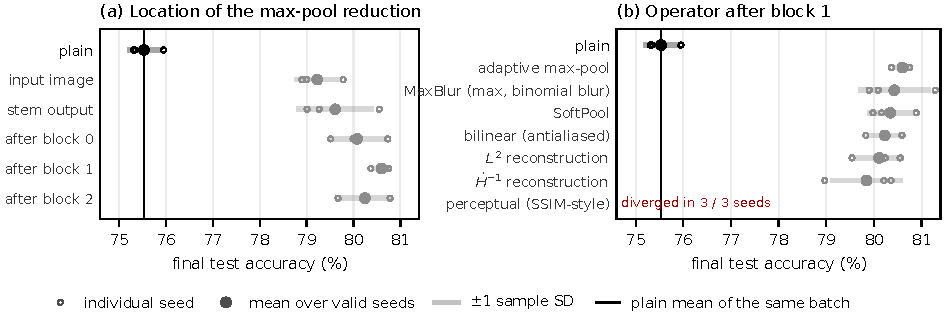
\includegraphics[width=\linewidth]{figures/appendix_resolution.pdf}
\caption{Resolution-only exploration with the $16\to24\to32$ schedule, three seeds per arm. Left: max-pooling insertion point. Right: reduction operator after block 1. The vertical line is this batch's plain mean; bars show sample SD. These scores guided selection on CIFAR-10.}
\label{fig:resolution}
\end{figure}
% GENERATED by paper/tools/make_paper_assets.py -- do not edit by hand.
% Sources: index configurations of resbench_resolution_only
% Provenance (configs, seeds, cells, files): paper/provenance/generated_assets.json
\begin{table}[!htbp]
\caption{Resolution-only batch (no additional Gaussian continuation): reduction operator at two locations, schedule $16\to24\to32$. Final test accuracy after 30 epochs, mean $\pm$ sample SD over three seeds. Plain arm of the batch: $75.53\pm0.36\%$. The perceptual operator after block 1 produced a non-finite loss in all three seeds.}
\label{tab:operators}
\centering\small
\begin{tabular}{@{}lcc@{}}
\toprule
Reduction operator & After block 1 (\%) & At the input (\%)\\
\midrule
Adaptive max-pool & $80.60\pm0.20$ & $79.23\pm0.48$\\
MaxBlur (max, binomial blur) & $80.43\pm0.75$ & $79.17\pm0.43$\\
SoftPool & $80.34\pm0.48$ & $79.28\pm0.46$\\
Bilinear (antialiased) & $80.23\pm0.38$ & $79.56\pm0.68$\\
$L^2$ reconstruction & $80.11\pm0.52$ & $79.64\pm0.33$\\
$\dot H^{-1}$ reconstruction & $79.85\pm0.76$ & $79.76\pm0.65$\\
Perceptual (SSIM-style) & Diverged (0/3 valid) & $79.98\pm0.40$\\
\bottomrule
\end{tabular}
\end{table}

Max-pooling after block 1 had the highest mean among its locations ($\rbMaxBOne\pm\rbMaxBOneSD\%$). The six valid operators at that point had overlapping seed ranges and none exceeded its mean (Table~\ref{tab:operators}). At the input, the perceptual and homogeneous $\dot H^{-1}$ reconstructions had higher means than max-pooling. We do not interpret these small differences as a definitive operator ranking.

For max-pooling, the progressive $16\to24\to32$ schedule scored above the tested delayed, shorter and reversed schedules. MaxBlur behaved differently: the reversed order gave $\rbMaxBlurReverse\%$, against $\rbMaxBlurProg\%$ for the progressive order. Keeping the reduced grid to the end gave $\rbFixedTwentyFour\%$ at 24 and $\rbFixedSixteen\%$ at 16. These controls retain a different inference computation, so they do not isolate restoration of resolution at equal inference cost. We retained adaptive max-pooling after block 1 as a simple, competitive operator.

\subsection{Final paired comparison}
The last selection batch contained 16 configurations and three seeds with matched assets. It compared plain, Gaussian placement, reduction locations and combinations with different per-site scale profiles.
\begin{figure}[htbp]\centering
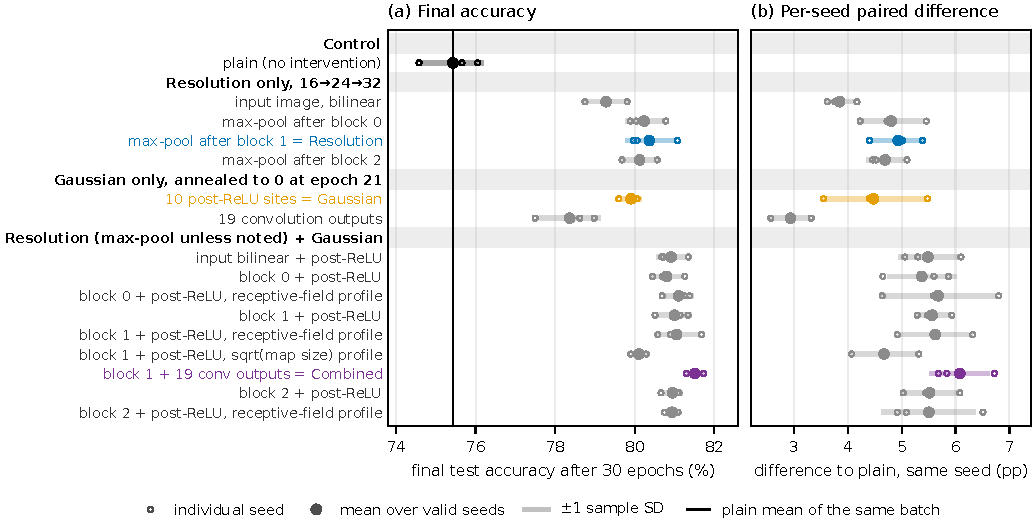
\includegraphics[width=\linewidth]{figures/appendix_unified.pdf}
\caption{All 16 configurations of the final selection batch. Left: final test accuracy. Right: difference to plain within the same seed. Colours identify the retained procedures. This is one internally paired batch; it does not remove the reuse of CIFAR-10 test performance during selection.}
\label{fig:unified}
\end{figure}
% GENERATED by paper/tools/make_paper_assets.py -- do not edit by hand.
% Sources: index configurations/cells of unified_selected
% Provenance (configs, seeds, cells, files): paper/provenance/generated_assets.json
\begin{table}[!htbp]
\caption{Retained procedures in the unified batch (\texttt{unified\_selected}, 48 runs). Final test accuracy after 30 epochs, where every procedure is in its target state (native resolution, no filter), so the current and target evaluations coincide. Mean $\pm$ sample SD over seeds 0--2. Same seed means the same pinned initial weights and data order, so gains are means of per-seed paired differences, with the sample SD of those differences in parentheses; neither is a confidence interval. Wall time is the mean per run, from model construction to the final summary, including per-epoch evaluation and checkpoint writes, two runs sharing a two-GPU Kaggle kernel (one T4 each).}
\label{tab:unified-reference}
\centering\small
\begin{tabular}{@{}lcccr@{}}
\toprule
Procedure & Test acc.\ (\%) & Seeds 0 / 1 / 2 & Gain over plain (pp) & Wall (s)\\
\midrule
Plain & $75.43\pm0.76$ & 74.58 / 75.66 / 76.05 & --- & 505\\
\methodR & $80.37\pm0.61$ & 79.97 / 80.06 / 81.07 & $+4.94$ ($0.50$) & 499\\
\methodG & $79.91\pm0.27$ & 80.06 / 80.06 / 79.60 & $+4.48$ ($0.97$) & 624\\
\methodRG & $81.51\pm0.22$ & 81.30 / 81.50 / 81.73 & $+6.08$ ($0.56$) & 733\\
\bottomrule
\end{tabular}
\end{table}

Without reduction, post-ReLU filtering scored above convolution-output filtering ($\uGauss\%$ versus $\uBlurConv\%$; paired difference $\uGaussMinusBlurConv\pm\uGaussMinusBlurConvSD$ points). With reduction after block 1, the order reversed: convolution-output filtering reached $\uComb\%$ against $\uResRelu\%$ for post-ReLU filtering, a paired difference of $\uCombMinusResRelu\pm\uCombMinusResReluSD$ points. Both differences were positive in all three seeds. Per-site scale profiles did not give a consistent further benefit; \uNearCombCount{} other combined arms finished within 0.6 points of the highest mean.

We selected one representative per family: max-pooling after block 1; the uniform Gaussian at ten post-ReLU sites; and max-pooling after block 1 with filtering at 19 convolution outputs. The uniform post-ReLU method was the better of the two basic Gaussian placements in this paired batch. It was not the highest mean among every historical Gaussian profile, and the selected procedures should not be called established family optima.



\begin{figure}[htbp]\centering
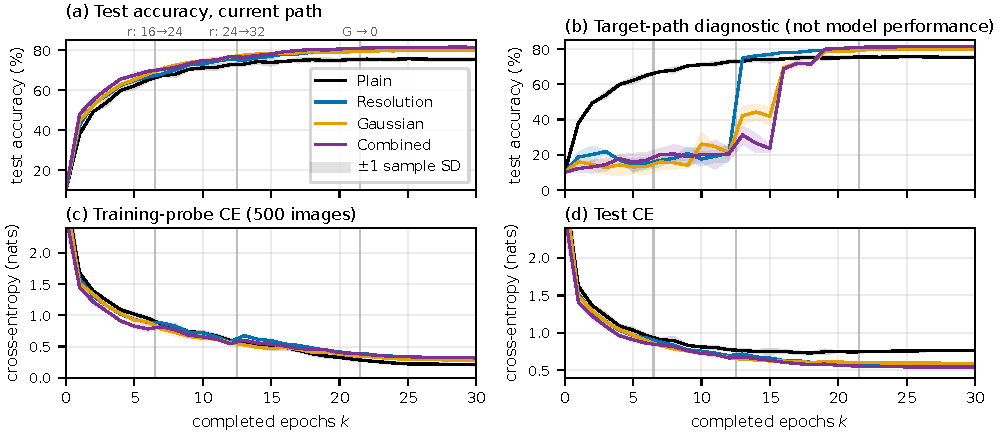
\includegraphics[width=\linewidth]{figures/appendix_unified_curves.pdf}
\caption{Selection-batch training records, means over three seeds. The current path retains the intervention of the epoch just completed; the target path removes it using saved BatchNorm statistics. Before restoration, the target diagnostic mixes the changed computation with a normalization-statistics mismatch. Training-probe CE uses 500 fixed images.}
\label{fig:unified-curves}
\end{figure}

\subsection{Other explored operators}
\label{app:alternatives}
SoftPool uses exponentially weighted local activations \citep{stergiou2021softpool}; MaxBlur combines max-pooling with binomial smoothing. The reconstruction operators address a different question: which low-resolution coefficients best reconstruct a channel $h$ through bilinear upsampling $U_r$? They minimize
\[
 \tfrac12(U_rz-h)^\top Q(U_rz-h),\qquad
 \mathbf1^\top(U_rz-h)=0,
\]
with $Q=I$ or the pseudoinverse of a spatial Laplacian. Unlike a TV constraint, this is a quadratic reconstruction objective on a smaller coefficient grid. The perceptual variant uses an SSIM-style reconstruction criterion; its divergence inside the network is retained as a failed experiment, not removed from the catalogue.

A one-seed db2 wavelet pilot on a 10,000-image subset reached $\xDbWave\%$ validation accuracy against $\xDbPlain\%$ for plain, at $\xDbWaveWall$\,s versus $\xDbPlainWall$\,s per run. Adaptive schedules and alternative allocations of time between blur levels did not clearly outperform fixed-schedule reruns in their one-seed study. Finally, longer one-seed Gaussian runs illustrate budget dependence: at 120 epochs, the convolution-output plateau schedule gave $\xLongLoPlateau\%$ against $\xLongLoPlain\%$ at the reference learning rate, and $\xLongHiPlateau\%$ against $\xLongHiPlain\%$ at ten times that rate. These exploratory controls are not equally tuned comparisons of the final three methods.
